\documentclass[onecolumn, draftclsnofoot,10pt, compsoc]{IEEEtran}
\usepackage{graphicx}
\usepackage{url}
\usepackage{setspace}
\usepackage{caption}
\setlength\parindent{0pt}

\usepackage{geometry}
\geometry{textheight=9.5in, textwidth=7in}
\graphicspath{{./}}

% 1. Fill in these details
\def \CapstoneTeamName{		TaalSquad}
\def \CapstoneTeamNumber{		33}
\def \GroupMemberOne{			Jonathan Buntin}
\def \GroupMemberTwo{			Aidan Carson}
\def \GroupMemberThree{			Manuel Lara-Navarro}
\def \GroupMemberFour{			Matthew Ruder}
\def \GroupMemberFive{			Pavel Shonka}
\def \GroupMemberSix{			Camden Sladcik}
\def \CapstoneProjectName{		The Autonomous Animal Locator}
\def \CapstoneSponsorCompany{	Levi Lab, Department of Fisheries and Wildlife, Oregon State University}
\def \CapstoneSponsorPerson{		Taal Levi}

% 2. Uncomment the appropriate line below so that the document type works
\def \DocType{		Design Document
				%Requirements Document
				%Technology Review
				%Design Document
				%Progress Report
				}
			
\newcommand{\NameSigPair}[1]{\par
\makebox[2.75in][r]{#1} \hfil 	\makebox[3.25in]{\makebox[2.25in]{\hrulefill} \hfill		\makebox[.75in]{\hrulefill}}
\par\vspace{-12pt} \textit{\tiny\noindent
\makebox[2.75in]{} \hfil		\makebox[3.25in]{\makebox[2.25in][r]{Signature} \hfill	\makebox[.75in][r]{Date}}}}
% 3. If the document is not to be signed, uncomment the RENEWcommand below
%\renewcommand{\NameSigPair}[1]{#1}

%%%%%%%%%%%%%%%%%%%%%%%%%%%%%%%%%%%%%%%
\begin{document}
\begin{titlepage}
    \pagenumbering{gobble}
    \begin{singlespace}
    	
\includegraphics[height=4cm]{coe_v_spot1}
        \hfill 
        % 4. If you have a logo, use this includegraphics command to put it on the coversheet.
        %\includegraphics[height=4cm]{CompanyLogo}   
        \par\vspace{.2in}
        \centering
        \scshape{
            \huge CS Capstone \DocType \par
            {\large\today}\par
            \vspace{.5in}
            \textbf{\Huge\CapstoneProjectName}\par
            \vfill
            {\large Prepared for}\par
            \Huge \CapstoneSponsorCompany\par
            \vspace{5pt}
            {\Large\NameSigPair{\CapstoneSponsorPerson}\par}
            {\large Prepared by }\par
            Group\CapstoneTeamNumber\par
            % 5. comment out the line below this one if you do not wish to name your team
            \CapstoneTeamName\par 
            \vspace{5pt}
            {\Large
                \NameSigPair{\GroupMemberOne}\par
                \NameSigPair{\GroupMemberTwo}\par
                \NameSigPair{\GroupMemberThree}\par
                \NameSigPair{\GroupMemberFour}\par
                \NameSigPair{\GroupMemberFive}\par
                \NameSigPair{\GroupMemberSix}\par
            }
            \vspace{20pt}
        }
        \begin{abstract}
The Autonomous Animal Locator (TAAL) is an automated drone to track vhf transmitters in remote locations. In order to do this we will use a receiver with frequency scanning, a drone designed specifically for tracking, and multiple software programs to display this information to the user as well as to automate the drone. This document shows the intended design and how all the components will be incorporated with each other.
	
        \end{abstract}    
    \end{singlespace}
\end{titlepage}
\newpage
\pagenumbering{arabic}
\tableofcontents
% 7. uncomment this (if applicable). Consider adding a page break.
%\listoffigures
%\listoftables
\clearpage

% 8. now you write!
\section{Overview}

\subsection{Scope}

The document describes the design of each component within The Autonomous Animal Locator (TAAL) application and how those components will be combined in order to deliver a complete product that will efficiently find and visualize animal locations.
The document will cover the design of the three components the team has identified as necessary to complete the project.
These are: the drone, the GUI, and the data processing.
\newline
\newline
The TAAL project can be applied to research, commercial, or individual projects that involve tracking of objects equipped with active VHF transmitters.
However, it is designed specifically to be able to track multiple targets over a large radius and in remote locations that are not required to have internet or cell reception.

\subsection{Purpose}

The TAAL project intends to solve the manual nature previously used to locate these animals, in which researchers must physically search and scan areas of up to 100 km${^{2}}$.
The scans can only locate a single animal at a time, and often require multiple days and/or more than one researcher to be able to effectively scan the whole forest.
The TAAL project will allow for a drastic reduction in both the man hours and number of researchers required to scan an equivalently sized area.

\subsection{Intended audience}

The TAAL project is intended for any person or team that is interested in locating one or several VHF transmitters within a large radius.
It provides a method within which researchers may deploy from a single central location and get approximate locations of transmitters within 100 km${^{2}}$ target area.

\section{Definitions}
\textbf{Drone}: An unmanned aerial vehicle. \newline
\textbf{ECE}: Electrical and Computer Engineering \newline
\textbf{GPS}: Global Positioning System. \newline
\textbf{GUI}: Graphical user interface. \newline
\textbf{Researcher}: A researcher is any user using this project for its intended purposes. \newline
\textbf{Storage Device}: A device used to store information or data. \newline
\textbf{TAAL}: The Autonomous Animal Locator. \newline
\textbf{Telemetry}: A method for collecting and transmitting GPS data from remote devices. \newline
\textbf{UI}: User interface. \newline
\textbf{VHF}: Very High Frequency. The transmitters used for the location of animals within the scope of this project broadcast in VHF.\newline


\section{Design Viewpoints}

\subsection{Context viewpoint}

The Context viewpoint illustrates services provided by the TAAL project.
Context is created by users that interact with the developed product.
It is a black box viewpoint that will showcase the common use cases.

\subsubsection{Design Concerns}

The Context viewpoint is used to single out the TAAL project's functionalities and the users that interact with them.
Concerns for the context viewpoint include: staying within the project's scope and detailing functionalities without too much technicality.

\subsubsection{Design Elements}

After completion, the drone should be able to carry out its autonomous mission to locate animals that are carrying VHF transmitters.
The drone will fly autonomously only after the user has defined its flight path, set the frequencies to listen for, and has given the command for the drone to start its mission.
It will then launch and fly along its flight path while scanning the proper radio frequencies; logging locational data while it flies.
Once the flight path has been completed, the drone will return to the user and land.
On return, the locational data collected by the drone will be transferred from the drone body to the researcher's field computer via a storage device.
Once all data has been imported to the field computer it will be processed and displayed visually.
The visualization of the data will be overlaid on the mission area map and will be at a maximum 50 m${^{2}}$ per animal location.
The drone may need to be launched multiple times to cover the desired area due to battery limitations.

\begin{figure}[h]

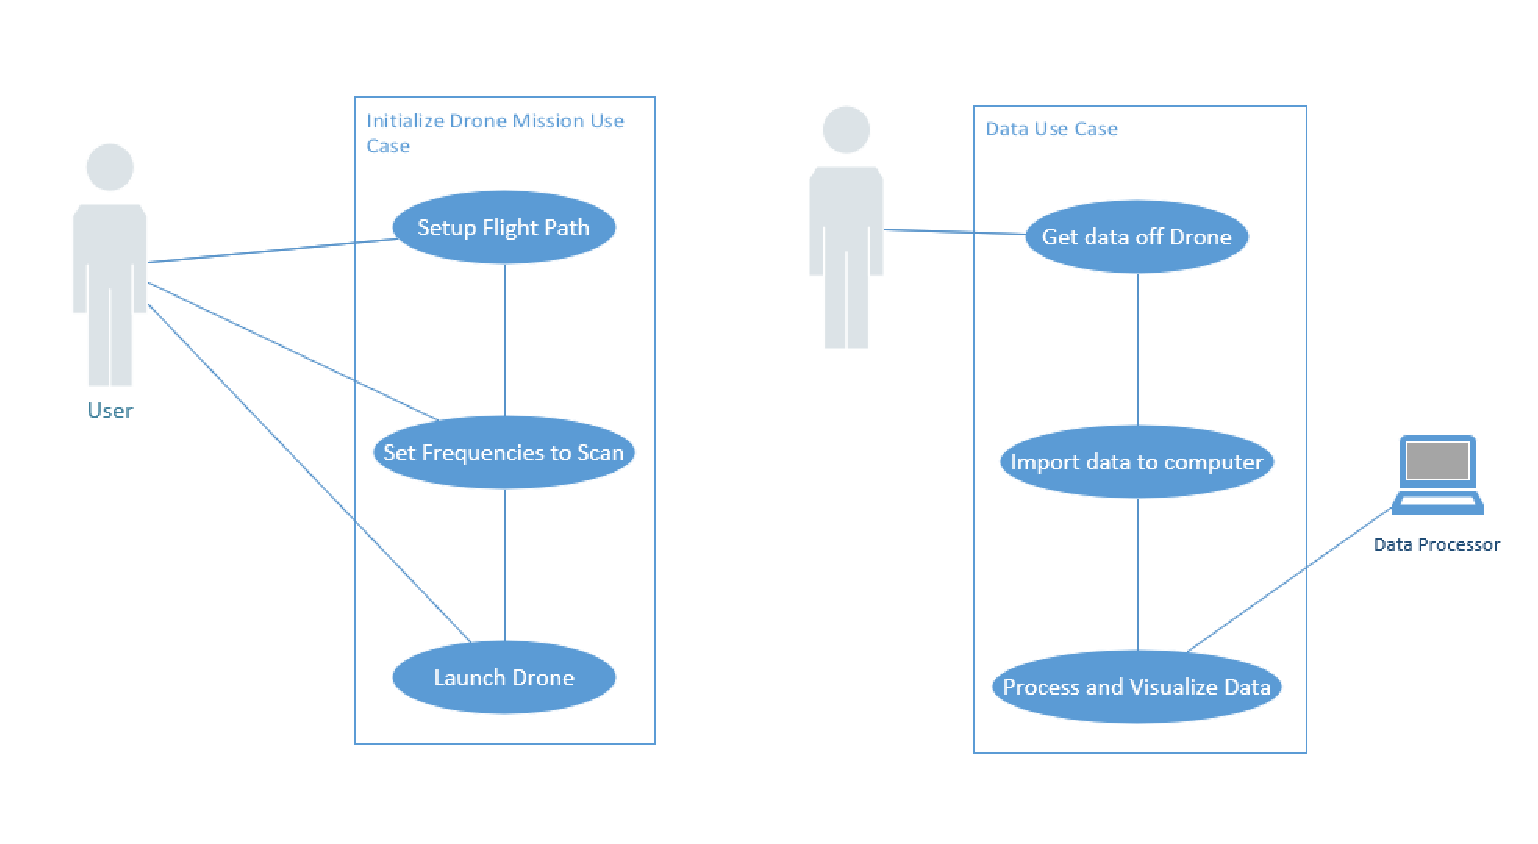
\includegraphics[width=7in]{useCase.eps}
\captionsetup{justification=centering}
\caption{UML Use Case Diagram}
\centering
\end{figure}

\subsection{Dependency viewpoint}

The dependency viewpoint of the TAAL project includes the hierarchy of components stemming from the top-level need for a drone to fly over a specified area.

\subsubsection{Design Concerns}

It is critical to the TAAL project to be able to locate VHF signals over a large area autonomously, and a drone with be built to accomplish this.
The drone will have three main components to deliver a functioning product: drone hardware, the UI software that will be used to program the drone as well as visualize data, and the aggregation, processing, and visualization of this data on top of the UI.
\newline
\newline
When physically constructing the hardware, servos, motors, and propellers must be installed in order for the drone to fly. There are many components that the frame depends on to properly deliver data relevant to the project goals. 
\newline
\newline
There must be a receiver for accepting VHF signals, a flight controller for autonomous flight, a storage device for storing the signal data received, and a telemetry device for real-time transmission back to the researcher.
\newline
\newline
For a working UI, software must be included for the researcher to be able to program and visualize a flight path, set the frequencies to search for, and program the drone.
A platform is needed that has the processing power to meet such requirements, as well as host the data processing software for when the location data is retrieved.
\newline
\newline
The data processing software must sufficiently translate the raw data given by the drone's receiver to a set of areas to indicate animal residence to an accuracy of 50m$^2$.
A platform is required with processing power capable of computing the raw data produced, as well as a language capable of making such sophisticated translations.

\subsubsection{Design Elements}

\textit{Design Entities}: 
\begin{itemize}
    \item drone body: flight controller, receiver, storage, telemetry.
    \item UI and data processor: desktop application, platform.
\end{itemize}
\textit{Design Relationships}: requires, uses, communicates with.\newline
\textit{Design Attributes}: name, type, dependencies, and resources.

\subsubsection{Dependencies attributes}

The drone hardware includes the drone body itself and all of the components it needs to fly - motors, servos, propellers, and power.
The purpose of the drone hardware is to provide housing for the internal components to scan for VHF antennae as well as to move the components in a large area for survey of a defined region.
It must be capable of carrying the hardware for location, and must therefore have the size and motors capable of delivering a non-zero payload.
Within the drone, in order to locate the VHF transmitter signals there must be a receiver and analog to digital converter.
The receiver will be the responsibility of the ECE team and will deliver a black box that given a VHF signal will output a GPS location, bearing of incoming signal, and time of receipt.
Our team will be responsible for storing that output to a local storage device
The drone will also need to have a telemetry system for transmitting back to the researcher at the ground station at all times.
The drone must also be capable of autonomous flight, using a flight controller to control its movement along a preprogrammed route allocated prior to the flight.
\newline
\newline
The UI software will be the point of contact between the researcher and the internal components of the drone, including the programming interface and visualization of received data.
It will need to be hosted on a platform that supports easy, offline access of the tools for programming the drone and visualizing the data.
A desktop application will most likely be in the solution.
The UI will be user-friendly and easy for a non-programmer to understand.
It will give the researcher visual feedback to allow for an area to be covered by the drone.
The software will then program the drone with a set of boundaries to survey the specified area.
Required is a module to communicate between the desktop application and the drone, either through a physical or wireless connection.
Once programmed, the drone will automatically take off, survey, and land at the original starting point.
\newline
\newline
The data processing component is responsible for taking raw data acquired from the drone during its flight and processing it into a form the researcher will be able to digest.
It is required to be hosted on a platform that supports the intensive calculations involved with transforming the data.
The application platform will be the same as the UI.
Data processing will occur after the drone has finished the flight.
From the central storage of the drone, the data will be transferred either through the means of a physical or wireless connection onto the desktop application.
From there, the output of the receiver that gives a GPS location, bearing, and timestamps of receipt of each signal will be transformed in the application into an estimated location of each animal projected over a downloaded map of the area.
\newline
\newline
\subsubsection{Example Languages}

The only languages that the project will require are in the development of the UI and the data processor.
The underlying application that contains these software components will need to be programmed as well.
Electron provides an efficient, simple, and cross-platform framework for building desktop applications in JavaScript and will be used.
For the UI, HTML, CSS, JavaScript, and the React.js framework will be used.
Python will be used for data processing because of their unique fit for making sophisticated translations into visualized data. 

\subsection{Interaction viewpoint}
The interaction viewpoint covers why, where, and how the different entities within the system communicate.
The different entities include the researcher, flight programming UI, flight controller, drone, receiver, storage device, and data processor.

\subsubsection{Design Concerns}
The concerns for the interaction viewpoint revolve around the different components of the complete system.
The concerns are what the different components are, with which components they interact, how they interact, and what information is passed between the components. 

\subsubsection{Design Elements}
There are seven components in this viewpoint, the researcher, flight programming UI, flight controller, drone, receiver, storage device, and data processor.
The first component of the system is the researcher. Researches will interact with the flight programming UI to set the coverage area and list which frequencies to search for.
Researchers will set the coverage area using a map and simply list the frequencies to search for.
The flight programming UI will then extrapolate flight instructions from the coverage area and send them to the flight controller.
In addition to sending the flight instructions to the flight controller, the frequencies list must be sent to the receiver.
The flight controller then pilots the drone using the flight commands provided to it and the information collected from its various sensors.
Frequency data from the flight programming UI will need to be sent to the receiver.
Data collected from the receiver has to be exported to the systems storage device.
The data must be formatted in a specific manner so that it is consistent for use by the software.
It must then be imported from the storage device to the data processor post flight.
The data processor will run the triangulation algorithm on the provided data and create a visual representation that is display to the researcher.

\subsection{Algorithm viewpoint}
The method used to locate each transmitter is a derivative of traditional triangulation.
\begin{figure}[h]
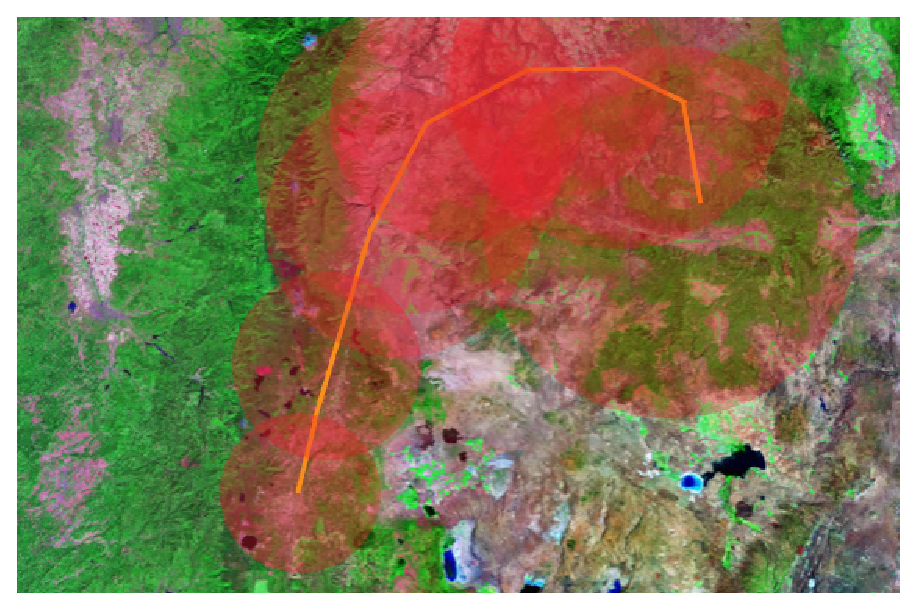
\includegraphics[width=7in]{satelliteMap.eps}
\captionsetup{justification=centering}
\caption{Graphical illustration of triangulation. The orange line illustrates theoretical flight path.}
\centering
\end{figure}
\subsubsection{Design Concerns}
The method used to translate the data into a graphical representation relies on the accuracy of the data received and researcher input for constants.
To construct each circle, the amplitude is used to determine the radius while position is determined by longitude, latitude, and altitude.
Due to the reliance on multiple pieces of information during the flight, the drone must collect accurate data in order for the system to work.
While this method can avoid the influence of minor outliers, too many outliers can skew the triangulated location of the transmitters.
Another issue is the reliance on the researcher to input the correct constants.
The radius of all the circles is controlled by an amplitude constant, which the researcher must manually set.
In addition, the opacity of each sphere is controlled by an opacity constant, which is also set by the researcher.
Sliders to control these constants shall alleviate the difficulty in calibrating the graphical representation of the data; however, the graphical representation is still reliant on the researcher's intuition in order to effectively calibrate and triangulate the final location of each transmitter.
\subsubsection{Design Elements}
The graphical projection of the data is presented using OpenGL.
Circles of a defined scale and opacity will be drawn onto a local satellite image. 

\begin{figure}[h]
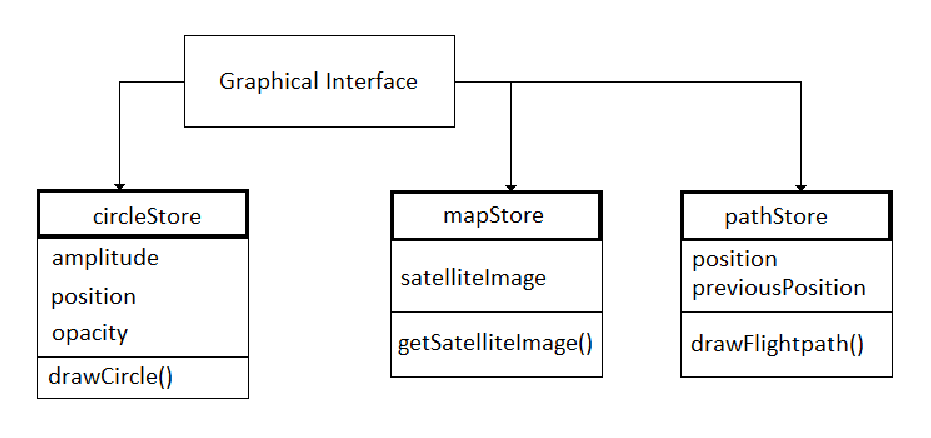
\includegraphics[width=7in]{GraphicsFlowchart.eps}
\captionsetup{justification=centering}
\caption{Flowchart diagram for graphical storage.}
\centering
\end{figure}

The position of each circle is defined using longitude, latitude, and altitude data acquired from the GPS module.
Each circle shall be connected by a line illustrating the flight path taken by the drone.
The radius of each circle is determined by the demodulated amplitude data acquired from the ECE team's receiver module.
Every circle's radius is scaled by the amplitude constant and the overall opacity of each circle is defined by the opacity constant.

\subsubsection{Processing attribute}
The graphical interface requires the receiver, drone, and GPS hardware to properly obtain data. The data collected will be processed all at once and displayed on a map for the researcher to view. The circles shall be graphically updated in real time as the researcher changes the opacity and amplitude constants.

\subsection{Resource viewpoint}

The Resource Viewpoint of the TAAL project includes the different resources and how they utilize each other. The different entities are the drone`s storage, power source and GPS, the signal receiver, and the researcher`s computer.

\subsubsection{Design Concerns}
Because of the limited battery life, we will need the majority of power concentrated for the motors. Therefore we need the minimum amount of processing to take place on the drone itself. Not only does this increase battery life, but it also mean less weight and size for the system - eliminating the ability of the drone to translate data in real time. Therefore data will need to be stored locally on the drone. A storage method will be required, we will use an SD card to hold the recorded data.
\newline
\newline
The drone should be able to detect when it should return to launch site due to low battery, by monitoring the battery level.
It will need to return to launch site to recharge before continuing the mission, therefore the battery should be easily removable or swapped.
There should be more than one battery available to minimize standby time during missions.
\newline
\newline
Storage should be able to hold all the data recorded for at least one mission.
The data will consist of a GPS location, bearing, and time-stamp at the receipt of each signal. It will be recorded for each frequency representing individual animals. The number of tracked animals should be able to change.
\newline
\newline
The station will be the user`s own mobile system, their personal computer or mobile device. The researcher`s system should be able to accept the drone`s storage device as input and have the desktop application installed.
The desktop application will process and read all of the receiver`s raw data.  

\subsubsection{Design Elements}
\textit{Design Entities}:
\begin{itemize}
    \item Drone: storage device(SD Card), Power Source, GPS.
	\item Receiver: Raw Data.
	\item Station: Software Application.
\end{itemize}
\textit{Design Relationships}:
\begin{itemize}
    \item Drone: 
    \begin{itemize}
        \item will need to read info from battery, GPS, and receiver.
        \item will need to write data to SD card
    \end{itemize}
    \item Station(researcher`s system):
    \begin{itemize}
        \item will need to program drone.
        \item will need to read data from drone`s storage device.
    \end{itemize}
\end{itemize}


\textit{Design Attributes}: 
    \begin{itemize}
        \item Battery life: will depend on motors and battery selected.
        \item SD card: Will depend on SD card size required.
        \item Station: will depend on the researcher`s system.
    \end{itemize}

\subsubsection{Resources Attribute}

Receiver will obtain signals from all the transmitters being tracked. This data will be recorded by the receiver and fed to the drone for storing. The receiver will be designed and develop by the ECE team. Data will be read and processed by the software application.  

\end{document}